\documentclass[12pt]{article}

\usepackage[utf8]{inputenc}	%Encoding UTF8 per accenti
\usepackage{pdflscape} % per pagine landscape

\usepackage[T1]{fontenc}

\usepackage[italian]{babel}

\usepackage[onehalfspacing]{setspace}	%Interlinea di 1.5

\usepackage[hyperfootnotes=false]{hyperref}	%Pacchetto per coll. ipertestuali

\usepackage{tabularx}
\usepackage{longtable,array} %Per Tabelle potenzialmente multipagina
\usepackage{fancyhdr}  % per gli header e footer
\usepackage{graphicx}  %per le immagini
\usepackage{flafter}
\usepackage{listings} %per i listati di codice
\usepackage[font=small,labelfont=bf]{caption}

\usepackage{framed}

\usepackage[headheight=2cm, headsep=0.5cm, a4paper, margin=3cm]{geometry}
\usepackage[bottom]{footmisc}

\hypersetup{colorlinks=true}		%Configurazione colore link documento
\hypersetup{linkcolor= blue}
\renewcommand\UrlFont{\color{blue}\rmfamily\itshape} %Forzato colore blu su tutti i link ESTERNI

\usepackage[dvipsnames,table]{xcolor}
\definecolor{bluelogo}{HTML}{415A66}
\definecolor{grigio}{HTML}{D0D0D0}
\usepackage{makecell}

\renewcommand{\footrulewidth}{0.1pt}
\newcommand{\glossario}{\textsubscript{G} }

\usepackage{fancyhdr}
\usepackage{lastpage}
 
\pagestyle{fancy}

\fancyhf{}

\lhead{
\includegraphics[scale=0.08]{./images/logo.png}}
\rhead{\rightmark}

\lfoot{Piano di Progetto v2.0.0}
\cfoot{}
\rfoot{Pagina \thepage \hspace{1pt} di \pageref*{LastPage}}

\makeindex
\setcounter{secnumdepth}{4}
\setcounter{tocdepth}{4}

%\lhead{
\includegraphics[scale=0.08]{./images/logo.png}}
%\usepackage[headheight=2cm, headsep=0.5cm, a4paper, margin=3cm]{geometry}

\newcolumntype{C}[1]{>{\centering\arraybackslash}m{#1}}
\usepackage{eurosym}

\usepackage{grffile}
\usepackage{float}



\begin{document}
\begin{titlepage}
\thispagestyle{empty}
\pagenumbering{gobble}

\begin{center}


\includegraphics[scale=0.3]{./images/logo.png} 

\large \textbf{Agents of S.W.E. - Progetto "G\&B"}
\vfill
\Huge \textbf{Allegato Tecnico}\\ \texbf{Product Baseline}\\ \normalsize 10 Aprile 2019
\vfill
\large
\renewcommand{\arraystretch}{1.3}
\begin{tabular}{r|l}
%\textbf{Versione} & 0.0.3\\
%\textbf{Approvazione} & ??\\
%\textbf{Redazione} & \parbox[t]{5cm}{Marco Chilese\\Luca Violato}\\
%\textbf{Verifica} & \parbox[t]{5cm}{??}\\
%%\textbf{Stato} & Work in Progress\\
%\textbf{Uso} & Esterno\\
\textbf{Destinato a} & \parbox[t]{5cm}{Agents of S.W.E. \\Prof. Tullio Vardanega\\Prof. Riccardo Cardin \\ Zucchetti S.p.A.}
\end{tabular}
\vfill
\small
\texttt{agentsofswe@gmail.com}
\end{center}
\end{titlepage}

\pagebreak

\pagenumbering{arabic}

%\section{Changelog}

\begin{center}
\begin{longtable}[c]{|m{.11\textwidth}|m{.13\textwidth}|m{.1\textwidth}|m{.19\textwidth}|p{.33\textwidth}|}
\hline
\rowcolor{bluelogo}\textbf{\textcolor{white}{Versione}} & \textbf{\textcolor{white}{Data}} & \textbf{\textcolor{white}{Autore}} & \textbf{\textcolor{white}{Ruolo}} & \textbf{\textcolor{white}{Descrizione}}\\
\hline \hline
\endfirsthead
0.0.1 & 2018-11-23 & Luca Violato & Amministratore & Strutturazione del Documento \\
\hline
\rowcolor{grigio} 0.0.2 & 2018-12-18 & Carlotta Segna & Responsabile & Standardizzazione tabella \\
\hline
\caption{Changelog del documento}
\end{longtable}
\end{center}
%\newpage


\tableofcontents

% Inclusione degli indici di tabelle e immagini
\listoftables
\listoffigures

\pagebreak

%\pagenumbering{arabic}

\section{Introduzione}\label{Intro}

\subsection{Scopo del Documento}
Il presente documento è stato realizzato con lo scopo di presentare le funzionalità del prodotto e spiegare, in modo intuitivo ma preciso, le modalità di utilizzo del plug-in \textit{G\&B}.

\subsection{Scopo del Prodotto}\label{ScopoProdotto}
Lo scopo del prodotto è la creazione di un plug-in per la piattaforma open source di visualizzazione e gestione dati, denominata \textit{Grafana}\glossario, con l'obiettivo di creare un sistema di alert\glossario dinamico per monitorare la "liveliness\glossario" del sistema a supporto dei processi DevOps\glossario e per consigliare interventi nel sistema di produzione del software. In particolare, il plug-in utilizzerà dati in input forniti ad intervalli regolari o con continuità, ad una rete bayesiana\glossario per stimare la probabilità di alcuni eventi, segnalandone quindi il rischio in modo dinamico, prevenendo situazioni di stallo.



\pagebreak

\section{Diagrammi di Package}

\subsection{Server - Diagrammi di Package}
\begin{figure}[H]
	\begin{center}
		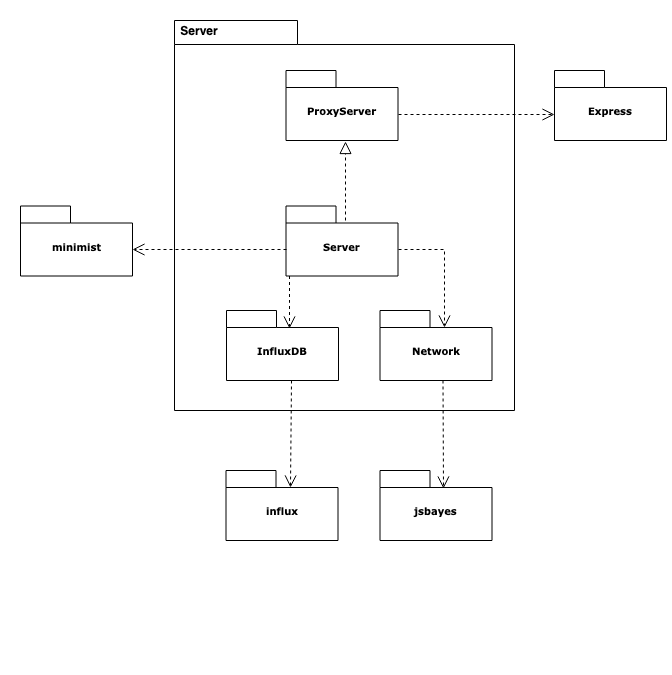
\includegraphics[scale=0.55]{./images/serverPackage.png} 
	\end{center}
	\caption{Diagramma dei package del Server}
\end{figure}



\subsection{Pannello - Diagrammi di Package}
	\begin{figure}[H]
		\begin{center}
			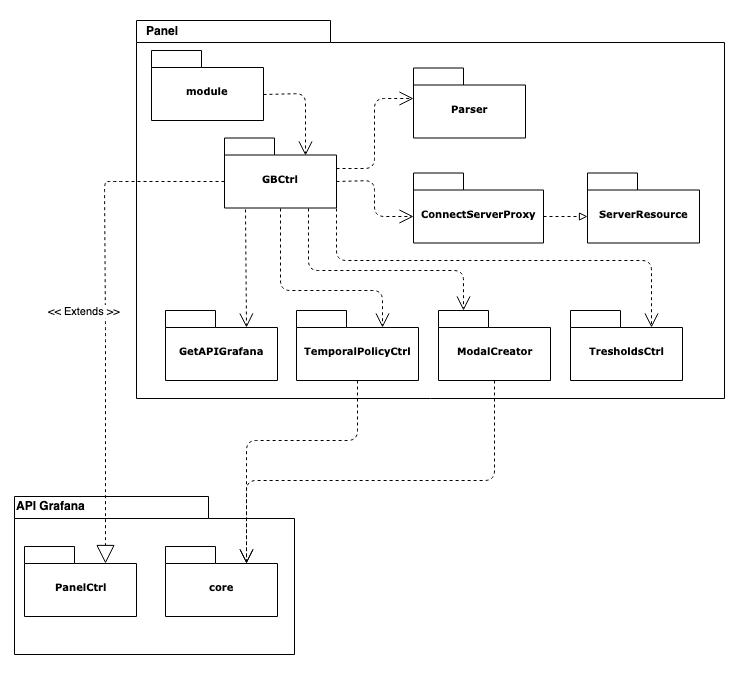
\includegraphics[scale=0.55]{./images/panelPackage.png} 
		\end{center}
	\caption{Diagramma dei package del Pannello}
	\end{figure}



\pagebreak

\begin{landscape}
	\section{Diagrammi delle Classi}
	\subsection{Server - Diagrammi delle Classi}
	\begin{figure}[H]
		\begin{center}
			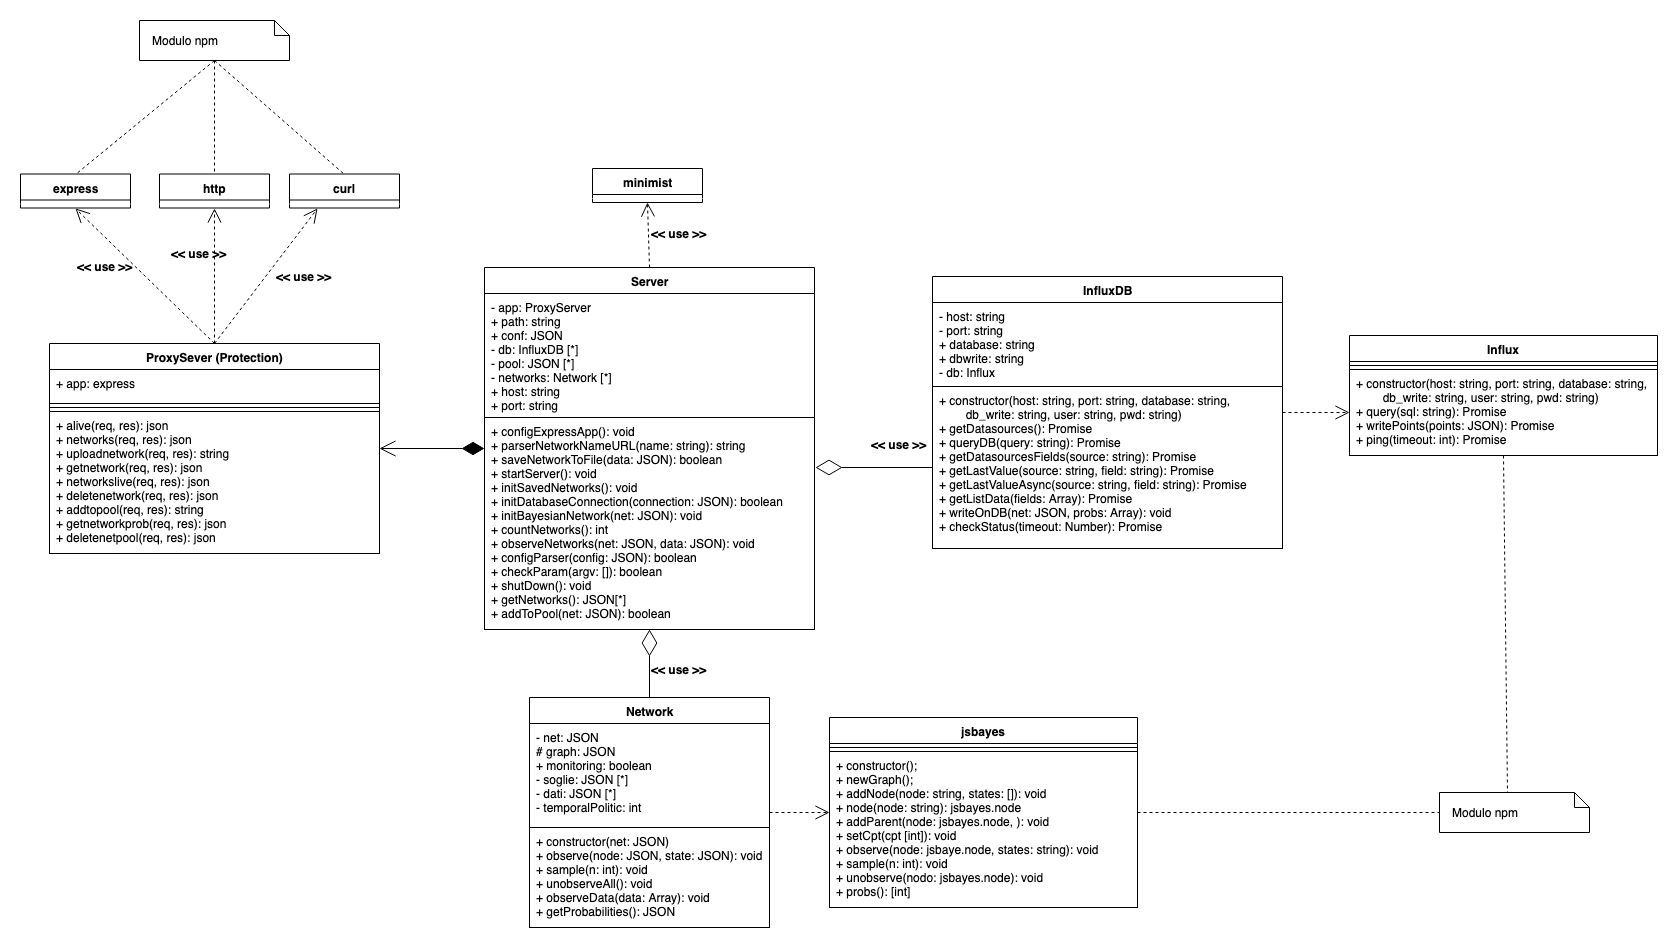
\includegraphics[scale=0.20]{./images/serverClassi.png} 
		\end{center}
		\caption{Diagramma delle classi del Server}
	\end{figure}
\end{landscape}

\begin{landscape}
	\subsection{Pannello - Diagrammi delle Classi}
\begin{figure}[H]
	\begin{center}
		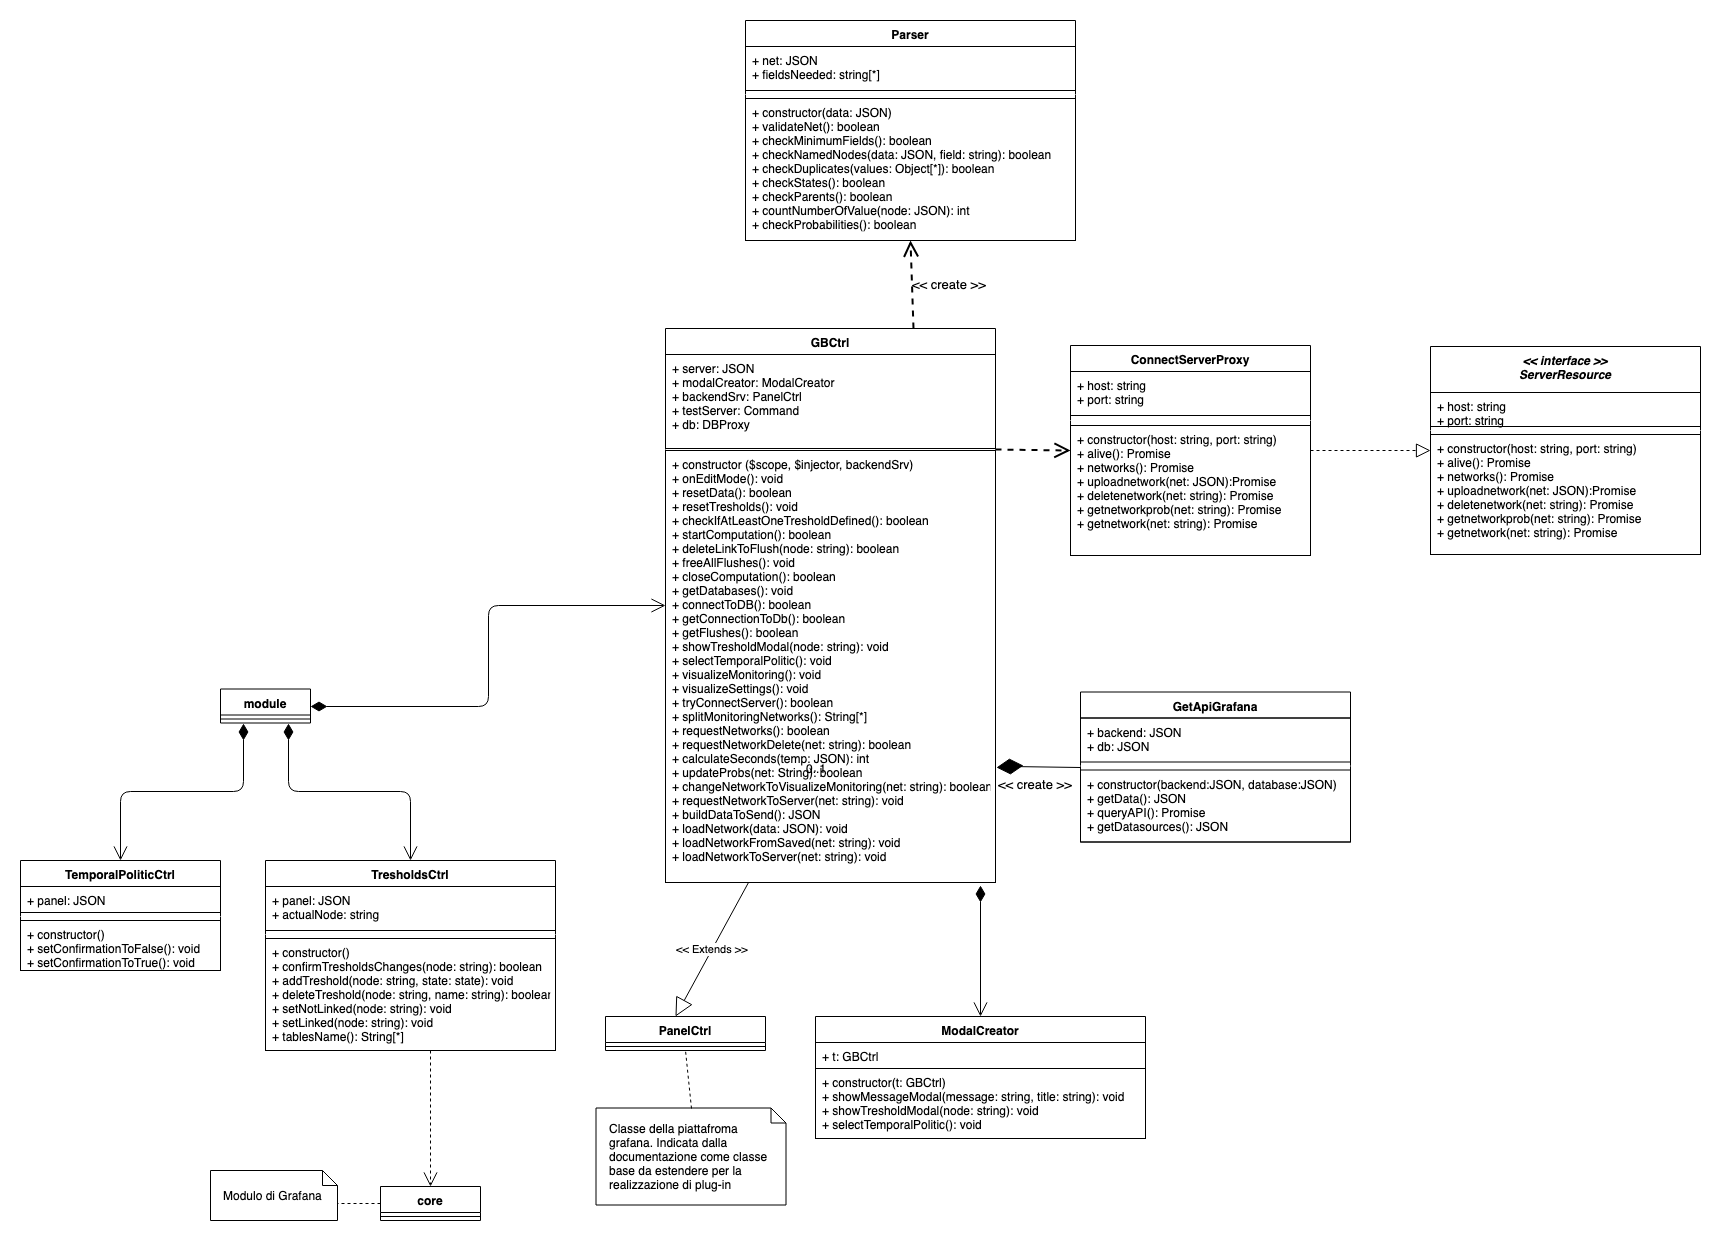
\includegraphics[scale=0.29]{./images/panelClassi.png} 
	\end{center}
	\caption{Diagramma delle classi del Pannello}
\end{figure}
\end{landscape}


\pagebreak

\begin{landscape}
	\section{Diagrammi di Sequenza}
	\subsection{Calcolo delle Probabilità}
\begin{figure}[H]
	\begin{center}
		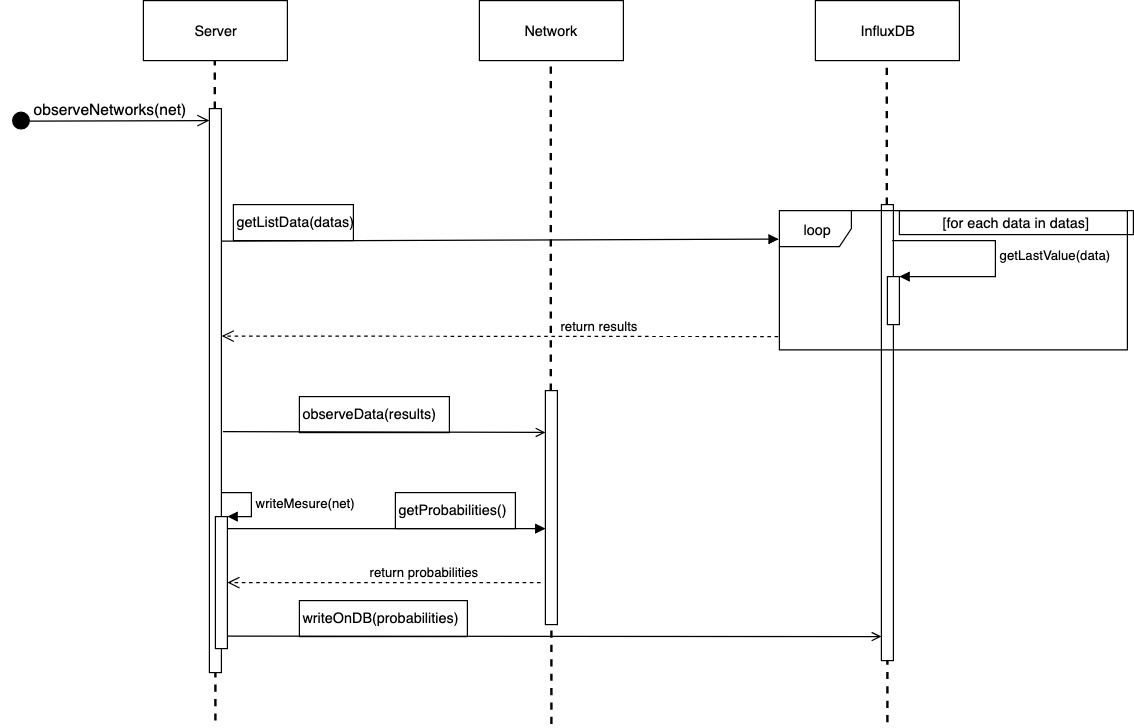
\includegraphics[scale=0.40]{./images/calocloProbSeq.png} 
	\end{center}
	\caption{Diagramma di sequenza che modella il calcolo delle probabilità}
\end{figure}
\end{landscape}

\begin{landscape}
	\subsection{Caricamento Rete}
	\begin{figure}[H]
		\begin{center}
			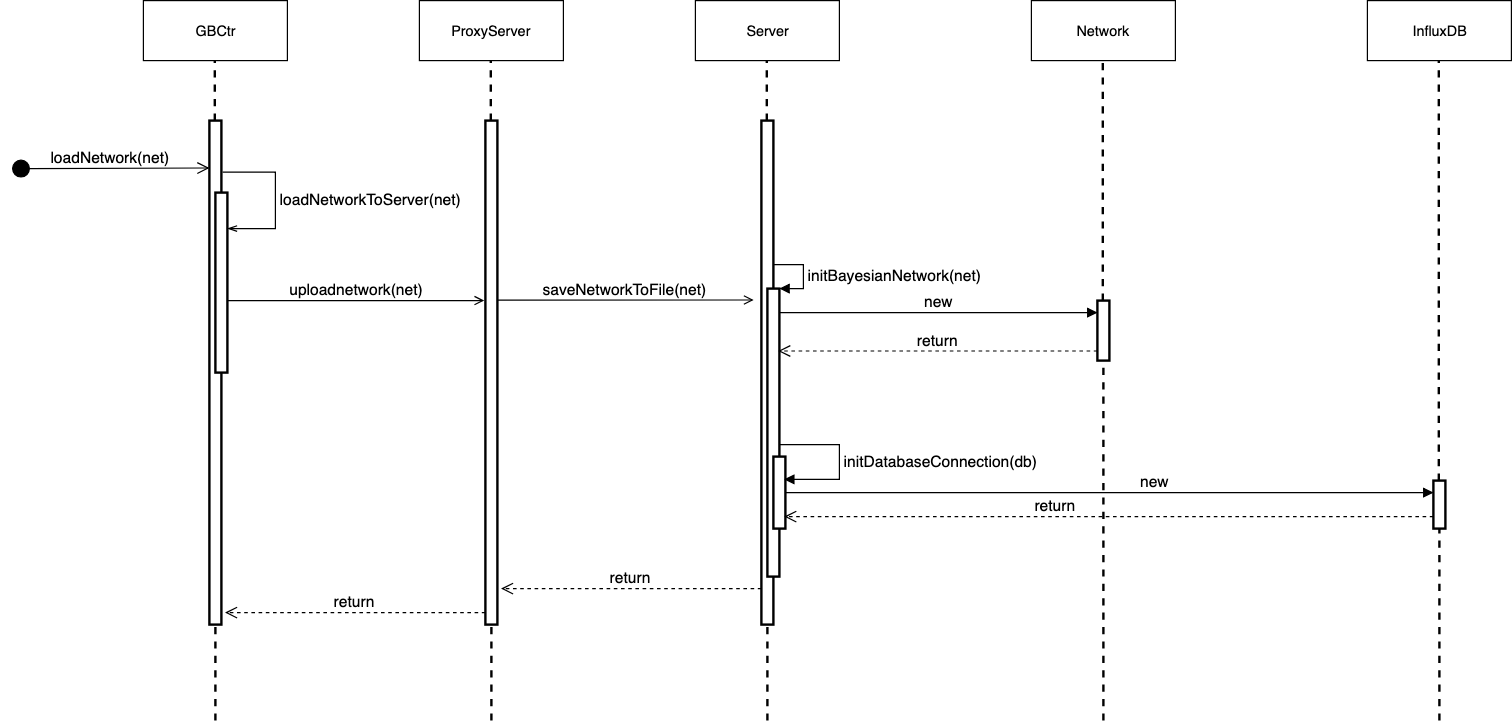
\includegraphics[scale=0.40]{./images/caricamentoReteSeq.png} 
		\end{center}
		\caption{Diagramma di sequenza che modella il caricamento della rete}
	\end{figure}
\end{landscape}



\end{document}